\section{Introduction}

This project focuses on building production-ready ELT (Extract, Load, Transform) data pipelines using Apache Airflow and dbt Cloud to process and analyze Airbnb and Census data for Sydney. The assignment demonstrates the implementation of a modern data engineering architecture following the medallion pattern (Bronze, Silver, Gold layers) and creates a comprehensive data warehouse with star schema design.

The datasets include 12 months of Airbnb listing data for Sydney (May 2020 to April 2021) and Australian Census data from 2016 at the Local Government Area (LGA) level. The goal is to create a robust data pipeline that can handle large-scale data processing while maintaining data quality and providing business insights through analytical data marts.

The project follows a four-part workflow using Apache Airflow for orchestration and dbt Cloud for data transformation, implementing a medallion architecture (Bronze, Silver, Gold layers) with star schema design. The detailed workflow is shown in Figure \ref{fig:project_workflow}.

\begin{figure}[H]
\centering
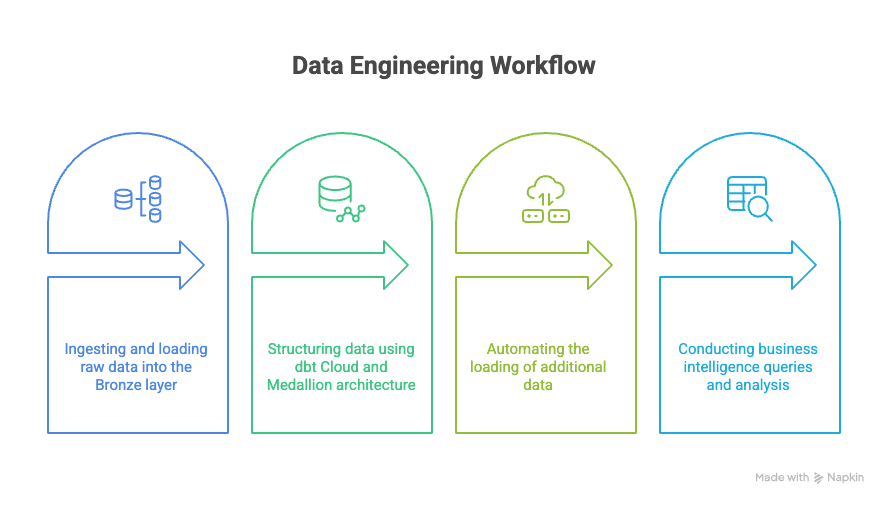
\includegraphics[width=0.9\textwidth]{images/project_workflow_diagram.png}
\caption{Project Workflow: Four-Part Data Engineering Pipeline}
\label{fig:project_workflow}
\end{figure}

This report serves as a handover document explaining the technical implementation, architectural decisions, data transformations, and current status of the pipeline. Each section includes detailed explanations of the data processing steps, challenges encountered, and solutions implemented.

\newpage

